\subsection*{Mass Matrix Training}

Figure \ref{fig:massnnloss} shows the training, validation and test loss during the training of the neural network.
As shown, the loss seems to converge to a very small error in all three cases, meaning that the neural network should effectively represent the mass of the manipulator if enough of the space was sampled uniformly.
One thing to note here was that Julia's RigidBodyDynamics package did not seem to honor the damping fields in the URDF files --- therefore, these training results show only the results when no friction was present in the system.

\begin{figure}[H]
  \centering
  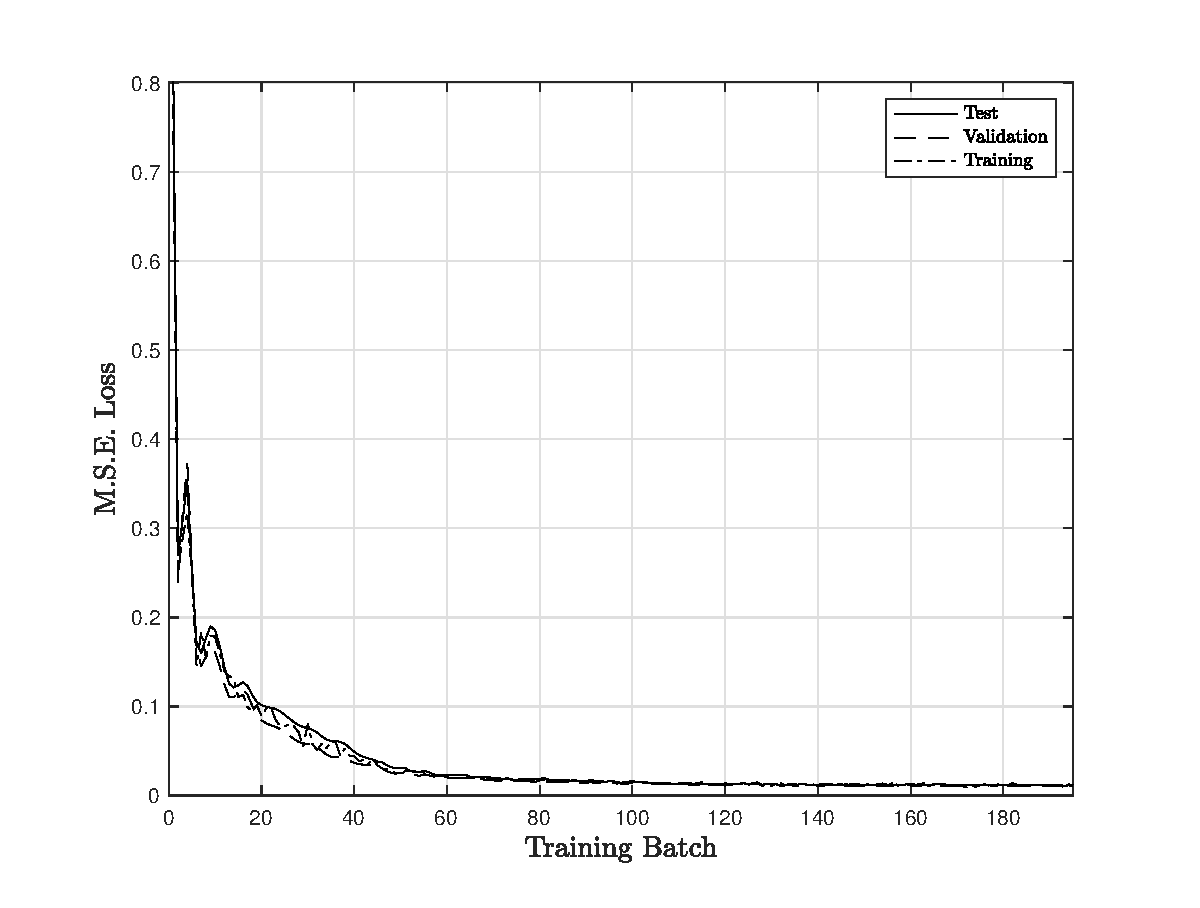
\includegraphics[width=0.80\textwidth]{figures/massnnloss_plot.eps}
  \caption{Mass Neural Network Cross Validation Loss Metrics}
  \label{fig:massnnloss}
\end{figure}

\subsection*{Kalman Filter}
Figure \ref{fig:kferror} shows the results of the Kalman filter when estimating the true position of the arm while moving through a trajectory.
All in all the results show about what is expected --- as more data samples are provided to the filter, the estimations improve.
One interesting note is the performance difference with and without the additional weight.
The margins of error are significantly smaller for the initial and home-bound trajectories than for the goal-bound trajectory when additional weight was present.
This is probably due to the failure in the dynamics when the additional weight was present.
The dynamics model used by RigidBodyDynamics was unable to accurately estimate the current acceleration when the additional weight was present, and this led to larger errors in the Kalman estimation.
Interestingly enough though, the values did still begin converging by the end of the simulation.

Another area to note is the sharp spikes in the estimation error.
These are most likely due to changing trajectory way-points.
The trajectories were built using linear interpolation between each point, so sharp spikes in the dynamics are probably present when traveling between the way-points provided during by the RRT* algorithm.
Even with these spikes, the error quickly settles, and still begins to converge.

\begin{figure}[H]
  \centering
  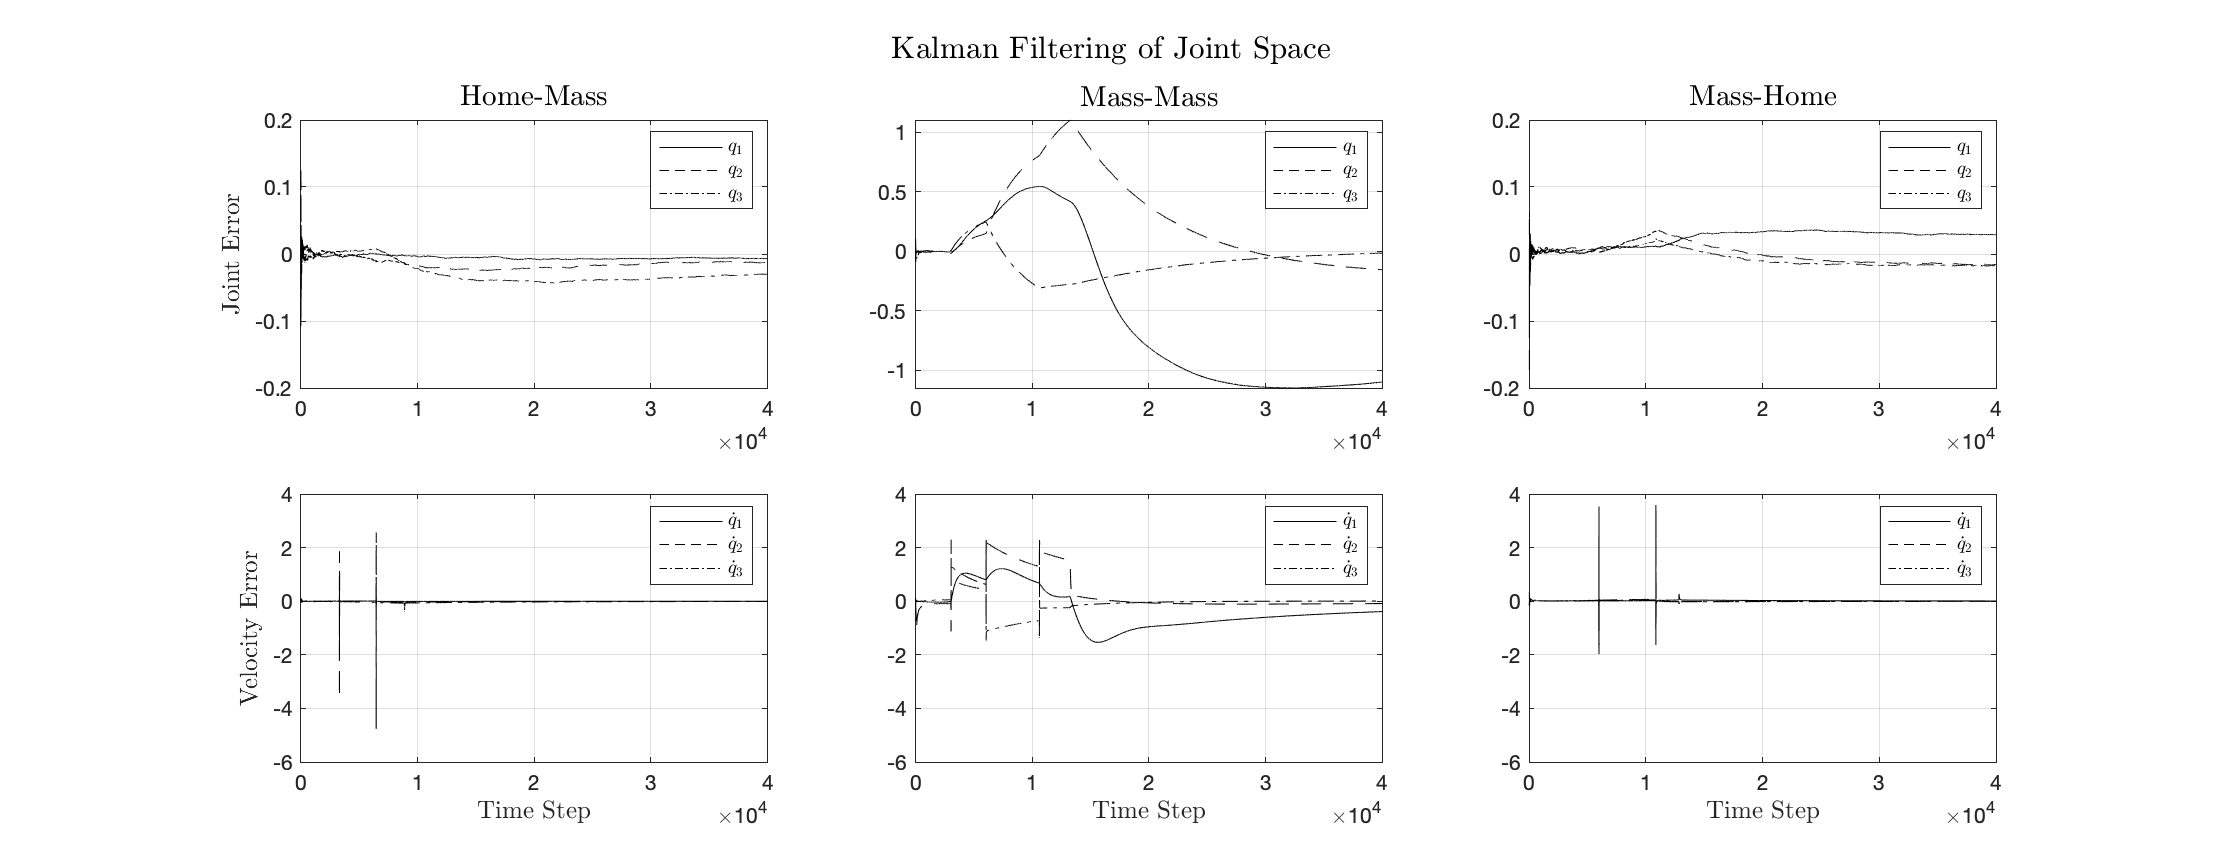
\includegraphics[width=\textwidth]{figures/kf_error.eps}
  \caption{Kalman filter prediction error during initial trajectory --- joint configurations and velocities.}
  \label{fig:kferror}
\end{figure}
